\clearpage
\section{02 ER Modelling: English Study Notes}\label{02_er_modelling_en}

CSC5041 · In-class Test 1 revision · 19 October 2026

\subsection{Scope and learning goals}\label{02_er_modelling_en-scope-and-learning-goals}

This chapter follows \hyperref[01_database_fundamentals_en]{01 Database Fundamentals}. It covers Week 2 on page 1 of the teaching plan and Question 1(a)--(b) on page 1 of Tutorial 1. The main source is the lecturer's \href{../../../slides/Week\%201B\%20-\%20Conceptual\%20DB\%20Design.pptx}{Week 1B - Conceptual DB Design.pptx}. All slide numbers below refer to their order in that file.

After studying this chapter, you should be able to identify entities, attributes, keys, and relationships from requirements; recognize weak entities; distinguish cardinality from participation; and draw ER diagrams using the lecture notation. Relational integrity constraints belong to Chapter 03; systematic ER-to-relational mapping belongs to Chapter 04. Explanatory supplements and original examples below do not establish additional examination requirements.

Slide 70 explicitly states: \textbf{``You must use the notation in the lecture for this course.''} This chapter uses the lecture's Chen-style notation rather than substituting crow's foot notation.

\subsection{1. What problem does ER modelling solve?}\label{02_er_modelling_en-what-problem-does-er-modelling-solve}

Source: slides 2--10, 54--56, and 69--70.

The Entity-Relationship model organizes application requirements into \textbf{entities, attributes, relationships, and constraints}. It belongs to conceptual design.

\begin{StudyCode}
Application requirements → identify objects and connections → ER diagram and constraints
                                                                       ↓ Chapter 04
                                                         relations and primary/foreign keys
\end{StudyCode}

For example, ``Every book must be published by exactly one publisher'' supplies two entity types, Book and Publisher; a relationship, PUBLISH; and a constraint requiring exactly one publisher for each book. Drawing two boxes and an unlabelled line omits the business rule.

Conceptual design first asks what information the application must express. This chapter does not begin with SQL table definitions or indexes, or mechanically add foreign keys as ER attributes.

\subsection{2. Entities, entity types, and entity sets}\label{02_er_modelling_en-entities-entity-types-and-entity-sets}

Source: slides 10--14 and 24--27.

\begin{longtable}[]{@{}
  >{\raggedright\arraybackslash}p{(\linewidth - 4\tabcolsep) * \real{0.3333}}
  >{\raggedright\arraybackslash}p{(\linewidth - 4\tabcolsep) * \real{0.3333}}
  >{\raggedright\arraybackslash}p{(\linewidth - 4\tabcolsep) * \real{0.3333}}@{}}
\toprule\noalign{}
\begin{minipage}[b]{\linewidth}\raggedright
Term
\end{minipage} & \begin{minipage}[b]{\linewidth}\raggedright
Meaning
\end{minipage} & \begin{minipage}[b]{\linewidth}\raggedright
Example
\end{minipage} \\
\midrule\noalign{}
\endhead
\bottomrule\noalign{}
\endlastfoot
Entity & A distinguishable physical or conceptual object & Amy, the student with ID S01 \\
Entity type & A definition of the common attributes and structure of a class of entities & Student with attributes sid, name, etc. \\
Entity set & The collection of entities of a type at a particular time & All students currently registered \\
Attribute & A property of an entity or relationship & A student's name; a grade for an enrolment \\
Domain / value set & The set of permitted values for an attribute & The allowed date values for an attribute \\
\end{longtable}

An entity type describes structure; an entity set describes current contents. Connect this distinction to schema versus instance in Chapter 01. Entities need not be physical objects: courses, accounts, and appointments can also be entities.

\textbf{Entity or attribute?} Ask whether the application must identify the object independently, record its own properties, and relate it to other objects. A publisher's name alone might be an attribute. If the application needs a publisher ID, publisher name, and the books it publishes, Publisher is better represented as an entity type. Being a noun alone does not make something an entity type.

\subsection{3. Attribute types: distinguish three dimensions}\label{02_er_modelling_en-attribute-types-distinguish-three-dimensions}

Source: slides 14--23 and 27--28.

\begin{longtable}[]{@{}
  >{\raggedright\arraybackslash}p{(\linewidth - 4\tabcolsep) * \real{0.3333}}
  >{\raggedright\arraybackslash}p{(\linewidth - 4\tabcolsep) * \real{0.3333}}
  >{\raggedright\arraybackslash}p{(\linewidth - 4\tabcolsep) * \real{0.3333}}@{}}
\toprule\noalign{}
\begin{minipage}[b]{\linewidth}\raggedright
Dimension
\end{minipage} & \begin{minipage}[b]{\linewidth}\raggedright
Type
\end{minipage} & \begin{minipage}[b]{\linewidth}\raggedright
Meaning and example
\end{minipage} \\
\midrule\noalign{}
\endhead
\bottomrule\noalign{}
\endlastfoot
Whether meaningful components are needed & Simple / atomic & Not subdivided in the current design, such as salary \\
Whether meaningful components are needed & Composite & Contains components with independent meanings, such as address(city, street, postcode) \\
Number of values per entity at one time & Single-valued & One dateOfBirth per student \\
Number of values per entity at one time & Multivalued & Several phoneNumber values per student \\
How the value is obtained & Stored & dateOfBirth is recorded directly \\
How the value is obtained & Derived & age is calculated from dateOfBirth and a reference date \\
\end{longtable}

These are not six mutually exclusive categories. An address can be \textbf{single-valued and composite}. If several addresses are allowed per person, it can be \textbf{multivalued and composite}. Slide 15 contrasts multivalued attributes with simple attributes; for clarity, assess decomposition and number of values separately. Simple and single-valued are not synonyms.

\subsubsection{Composite versus multivalued}\label{02_er_modelling_en-composite-versus-multivalued}

\begin{StudyCode}
Composite:   one address = (city, street, postcode)
Multivalued: phone numbers = {130..., 131...}
\end{StudyCode}

Branches from a composite attribute describe \textbf{components}. A double oval means that an entity may have \textbf{more than one value} for the attribute. Slide 21 explains that subdivision is unnecessary if an address is used only as a whole; the choice depends on the operations required.

\subsubsection{Stored versus derived}\label{02_er_modelling_en-stored-versus-derived}

Age depends on date of birth and a reference date. Manually updating age can make it inconsistent with the birth date, so the lecture's conceptual treatment uses age as a derived attribute and dateOfBirth as a stored attribute. This describes the conceptual meaning, not a required caching implementation for a real product.

\subsubsection{Missing values: NULL}\label{02_er_modelling_en-missing-values-null}

Slide 28 uses NULL for an unknown or inapplicable attribute value: a person's height may be unknown, or a person may have no college degree. NULL is not the number zero or a known empty string. SQL comparisons involving NULL belong to Chapter 06.

\subsection{4. Keys: check uniqueness and minimality separately}\label{02_er_modelling_en-keys-check-uniqueness-and-minimality-separately}

Source: slides 29--32.

\begin{longtable}[]{@{}
  >{\raggedright\arraybackslash}p{(\linewidth - 2\tabcolsep) * \real{0.5000}}
  >{\raggedright\arraybackslash}p{(\linewidth - 2\tabcolsep) * \real{0.5000}}@{}}
\toprule\noalign{}
\begin{minipage}[b]{\linewidth}\raggedright
Type
\end{minipage} & \begin{minipage}[b]{\linewidth}\raggedright
Definition
\end{minipage} \\
\midrule\noalign{}
\endhead
\bottomrule\noalign{}
\endlastfoot
Superkey & A set of attributes that uniquely identifies an entity; redundant attributes are allowed \\
Candidate key & A minimal superkey: removing any attribute destroys the guarantee of uniqueness \\
Primary key & A candidate key selected by the designer \\
Composite key & A key consisting of more than one attribute \\
\end{longtable}

\textbf{Minimal does not mean minimum size.} A type can have both a one-attribute candidate key and a two-attribute candidate key, provided neither contains a redundant attribute.

\textbf{Original example:} suppose both sid and email are guaranteed unique in Student.

\begin{itemize}
\tightlist
\item
  \texttt{\{sid\}} and \texttt{\{email\}} are candidate keys; \texttt{\{sid\}} may be selected as the primary key.
\item
  \texttt{\{sid,\ name\}} is a superkey but not a candidate key, because name is redundant.
\item
  Three current students having different names does not establish \texttt{\{name\}} as a key. A key must be unique in every state permitted by the requirements.
\end{itemize}

Components of a composite key need not be individually unique. If a local number is unique only within its region, \texttt{\{regionCode,\ localNumber\}} may jointly identify an object. A key containing several attributes is not a multivalued attribute.

An artificial identifier can be introduced when natural attributes cannot reliably distinguish objects. Adding an ID does not by itself express all other business constraints.

\Needspace{11cm}
\subsection{5. Strong entities, weak entities, and partial keys}\label{02_er_modelling_en-strong-entities-weak-entities-and-partial-keys}

\StudyVisual{weak}{en}

Source: slides 33--35; local numbering also appears in Tutorial 1, Question 1(a).

\begin{longtable}[]{@{}
  >{\raggedright\arraybackslash}p{(\linewidth - 2\tabcolsep) * \real{0.5000}}
  >{\raggedright\arraybackslash}p{(\linewidth - 2\tabcolsep) * \real{0.5000}}@{}}
\toprule\noalign{}
\begin{minipage}[b]{\linewidth}\raggedright
Term
\end{minipage} & \begin{minipage}[b]{\linewidth}\raggedright
Identification rule
\end{minipage} \\
\midrule\noalign{}
\endhead
\bottomrule\noalign{}
\endlastfoot
Strong entity & Has its own key and can be identified independently \\
Weak entity & Lacks a complete key of its own; identification requires the owner's identifier and its own partial key \\
Owner entity & Supplies the context required to identify a weak entity \\
Partial key / discriminator & Distinguishes weak entities belonging to the same owner, without guaranteeing uniqueness across owners \\
Identifying relationship & Connects a weak entity to its owner \\
\end{longtable}

The phrase ``partially unique'' on slide 34 should be read as \textbf{unique within an owner's scope}. It does not mean that the key identifies only some of the entity's attributes.

\subsubsection{A chain with two weak entity types}\label{02_er_modelling_en-a-chain-with-two-weak-entity-types}

The following explains the numbering rules in Tutorial 1; it is not a complete solution to the tutorial.

\begin{StudyCode}
Owner: ownerID is globally unique
  └─ Pet: petNo is unique only within that Owner
       └─ Treatment: treatmentNo is unique only within that Pet

Full identifier of Pet       = (ownerID, petNo)
Full identifier of Treatment = (ownerID, petNo, treatmentNo)
\end{StudyCode}

Pet has partial key petNo; Treatment has partial key treatmentNo. Treatment's immediate owner, Pet, is itself weak, so identification must follow the owner chain to obtain the full context.

Here each Pet belongs to exactly one Owner, and each Treatment belongs to exactly one Pet. A weak entity has \textbf{total participation} in its identifying relationship. This does not imply that every owner must have a weak entity. Tutorial 1 explicitly requires each Owner to have at least one Pet, but does not require every Pet to have a Treatment.

\textbf{Clarifying the slides:} ``a weak entity does not have its own primary key'' means that it lacks an \textbf{independent complete key of its own}. A relation produced later can still have a primary key combining the owner key and partial key; Chapter 04 covers that mapping.

\textbf{Dependency alone does not establish weakness.} An employee may be required to work in a department, but can still be strong if empID identifies the employee independently. The issue is dependence on the owner for identification.

\subsection{6. Relationships, relationship attributes, and roles}\label{02_er_modelling_en-relationships-relationship-attributes-and-roles}

Source: slides 38--42 and 48--53.

A relationship type describes an association between entities. A relationship instance contains particular participants. ENROLLED\_IN(Student, Course) is a relationship type; ``S01 takes C01'' is an instance.

\subsubsection{Where should an attribute go?}\label{02_er_modelling_en-where-should-an-attribute-go}

In the WORKS\_ON example on slide 48, fraction is the proportion of a researcher's time devoted to a particular project:

\begin{StudyCode}
(Researcher R1, Project P1) → fraction = 0.4
(Researcher R1, Project P2) → fraction = 0.6
\end{StudyCode}

The value describes a \textbf{particular researcher--project combination}, so it belongs to WORKS\_ON. Attaching it only to Researcher would not distinguish projects; attaching it only to Project would not distinguish researchers. Similarly, borrowing dates describe a borrowing association.

\subsubsection{Several relationships can connect the same types}\label{02_er_modelling_en-several-relationships-can-connect-the-same-types}

In Tutorial 1, Clinic and Veterinarian participate in both WORKS\_AT and MANAGES. Employment and management have different meanings and should not become a single unlabelled line.

``The manager must work at that clinic'' further requires \textbf{every MANAGES pair to also be a WORKS\_AT pair}. Drawing both relationships and assigning their individual cardinalities does not fully express this rule; add a written constraint.

\subsubsection{Roles and relationship degree}\label{02_er_modelling_en-roles-and-relationship-degree}

A binary relationship has two participating roles; a ternary relationship has three. Slide 50 illustrates Researcher, Student, and Course. Slide 53 shows one Person type participating in separate Student and Researcher roles.

\textbf{Explanatory supplement:} the number of roles need not equal the number of distinct entity types. EMPLOYEE can participate in SUPERVISES as both supervisor and subordinate, giving a binary recursive relationship. Label roles when a type participates more than once.

Slide 52 advises beginners to try binary representations. This is a modelling heuristic, \textbf{not a theorem that every ternary relationship can be decomposed without loss into three binary relationships}. Check whether the original association among all three participants can still be recovered. This chapter mainly focuses on binary relationships.

\subsection{7. Cardinality constraints: ask about both maxima}\label{02_er_modelling_en-cardinality-constraints-ask-about-both-maxima}

Source: slides 43--45.

For a binary relationship A---R---B, fix one A and then one B, and ask how many entities on the other side each can be associated with at most.

\begin{longtable}[]{@{}
  >{\raggedright\arraybackslash}p{(\linewidth - 4\tabcolsep) * \real{0.3333}}
  >{\raggedright\arraybackslash}p{(\linewidth - 4\tabcolsep) * \real{0.3333}}
  >{\raggedright\arraybackslash}p{(\linewidth - 4\tabcolsep) * \real{0.3333}}@{}}
\toprule\noalign{}
\begin{minipage}[b]{\linewidth}\raggedright
Cardinality ratio A:B
\end{minipage} & \begin{minipage}[b]{\linewidth}\raggedright
Maximum B entities for one A
\end{minipage} & \begin{minipage}[b]{\linewidth}\raggedright
Maximum A entities for one B
\end{minipage} \\
\midrule\noalign{}
\endhead
\bottomrule\noalign{}
\endlastfoot
1:1 & One & One \\
1:N & Many & One \\
M:N & Many & Many \\
\end{longtable}

\textbf{Original example:} a Department can have many Employees, and each Employee belongs to at most one Department. Therefore Department:Employee is 1:N.

The lecture's Chen notation is \texttt{Department\ —\ 1\ —\ WORKS\_FOR\ —\ N\ —\ Employee}. \textbf{The 1 beside Department does not mean one employee per department.} It means at most one Department for a given Employee. Write the two verbal statements before positioning the labels.

The example on slides 44--45 works the same way: a Grant supports only one Project, while a Project can receive support from many Grants. Thus Project:Grant = 1:N, or Grant:Project = N:1 when the order is reversed.

\texttt{N} and \texttt{M} permit many; they do not specify an exact current count or require at least two. \textbf{A 1:N ratio alone does not say that every employee must have a department.}

\subsection{8. Participation constraints: ask about both minima}\label{02_er_modelling_en-participation-constraints-ask-about-both-minima}

Source: slides 46--47; notation on slide 57.

\begin{longtable}[]{@{}
  >{\raggedright\arraybackslash}p{(\linewidth - 4\tabcolsep) * \real{0.3333}}
  >{\raggedright\arraybackslash}p{(\linewidth - 4\tabcolsep) * \real{0.3333}}
  >{\raggedright\arraybackslash}p{(\linewidth - 4\tabcolsep) * \real{0.3333}}@{}}
\toprule\noalign{}
\begin{minipage}[b]{\linewidth}\raggedright
Constraint
\end{minipage} & \begin{minipage}[b]{\linewidth}\raggedright
Requirement for each entity of the type
\end{minipage} & \begin{minipage}[b]{\linewidth}\raggedright
Lecture notation
\end{minipage} \\
\midrule\noalign{}
\endhead
\bottomrule\noalign{}
\endlastfoot
Total participation & Must participate in at least one relationship instance & Double line between entity and relationship \\
Partial participation & May participate in none; the minimum is zero & Single line \\
\end{longtable}

Partial participation does not require some entities to remain uninvolved; it \textbf{allows} that possibility. Every current entity participating is not evidence that the rules require total participation.

Combining minima and maxima helps check the design. The following \texttt{(\allowbreak{}min,\allowbreak{}max)\allowbreak{}} notation is a reading aid for written tables. Formal diagrams still use the lecture's cardinality labels and single/double lines.

\begin{longtable}[]{@{}ll@{}}
\toprule\noalign{}
Wording & Participation count for the entity under discussion \\
\midrule\noalign{}
\endhead
\bottomrule\noalign{}
\endlastfoot
Zero or one / at most one & (0,1) \\
Exactly one & (1,1) \\
Zero or more & (0,N) \\
One or more / at least one & (1,N) \\
\end{longtable}

Suppose every Employee must work in exactly one Department, but a Department may temporarily have no Employees. Employee has \texttt{(\allowbreak{}1,\allowbreak{}1)\allowbreak{}} and Department has \texttt{(\allowbreak{}0,\allowbreak{}N)\allowbreak{}}. Department:Employee is 1:N; Employee participates totally and Department participates partially.

\textbf{Watch the direction:} an entity's \texttt{(\allowbreak{}min,\allowbreak{}max)\allowbreak{}} above counts its possible counterparts. This is a different reading convention from the placement of Chen cardinality labels. Do not copy positions mechanically.

\subsection{9. Lecture notation reference}\label{02_er_modelling_en-lecture-notation-reference}

Source: slides 35--37, 45, 47, and 57; the original diagrams were visually inspected.

\begin{longtable}[]{@{}
  >{\raggedright\arraybackslash}p{(\linewidth - 2\tabcolsep) * \real{0.5000}}
  >{\raggedright\arraybackslash}p{(\linewidth - 2\tabcolsep) * \real{0.5000}}@{}}
\toprule\noalign{}
\begin{minipage}[b]{\linewidth}\raggedright
Meaning
\end{minipage} & \begin{minipage}[b]{\linewidth}\raggedright
Symbol
\end{minipage} \\
\midrule\noalign{}
\endhead
\bottomrule\noalign{}
\endlastfoot
Regular / strong entity type & Single rectangle \\
Weak entity type & Double rectangle \\
Regular relationship type & Single diamond \\
Identifying relationship & Double diamond \\
Regular attribute & Single oval \\
Key attribute & Solid underline under the name; indicate all components of a composite key \\
Partial key & Dashed underline under the name, illustrated on slide 35 \\
Multivalued attribute & Double oval \\
Composite attribute & An oval connected to ovals for its components \\
Derived attribute & Dashed oval \\
Total / partial participation & Double / single line \\
Cardinality ratio & Labels 1, N, or M at the relationship ends \\
\end{longtable}

Double rectangles, diamonds, ovals, and connecting lines have different meanings. \textbf{A double line means total participation, not many-to-many. A double oval means multivalued, not composite.} An underline for a key is also different from the dashed boundary of a derived attribute.

\subsection{10. Worked example: library requirements to an ER diagram}\label{02_er_modelling_en-worked-example-library-requirements-to-an-er-diagram}

Source: slides 58--68. The following restates the lecture requirements and provides a study redraw; it is not a new practice examination question.

\subsubsection{Step 1: entities and attributes}\label{02_er_modelling_en-step-1-entities-and-attributes}

\begin{longtable}[]{@{}lll@{}}
\toprule\noalign{}
Entity type & Key & Other attributes \\
\midrule\noalign{}
\endhead
\bottomrule\noalign{}
\endlastfoot
Book & bookID & title, price, availability \\
Reader & readerID & name, phoneNumber, address(street, suburb) \\
Publisher & publisherID & name \\
Author & authorID & name, phoneNumber, dateOfBirth \\
\end{longtable}

The full requirements on slides 58--60 do not give Reader a birth date, although the step-by-step example on slide 62 introduces dob. This chapter follows the full requirements and final diagram on slide 68, omitting Reader.dob. Author's date of birth is explicitly required. This is a local inconsistency in the slides, not a reason to silently add a requirement.

\subsubsection{Step 2: state each relationship in both directions}\label{02_er_modelling_en-step-2-state-each-relationship-in-both-directions}

\begin{longtable}[]{@{}
  >{\raggedright\arraybackslash}p{(\linewidth - 8\tabcolsep) * \real{0.2000}}
  >{\raggedright\arraybackslash}p{(\linewidth - 8\tabcolsep) * \real{0.2000}}
  >{\raggedright\arraybackslash}p{(\linewidth - 8\tabcolsep) * \real{0.2000}}
  >{\raggedright\arraybackslash}p{(\linewidth - 8\tabcolsep) * \real{0.2000}}
  >{\raggedright\arraybackslash}p{(\linewidth - 8\tabcolsep) * \real{0.2000}}@{}}
\toprule\noalign{}
\begin{minipage}[b]{\linewidth}\raggedright
Relationship
\end{minipage} & \begin{minipage}[b]{\linewidth}\raggedright
Counterparts for each left entity
\end{minipage} & \begin{minipage}[b]{\linewidth}\raggedright
Counterparts for each right entity
\end{minipage} & \begin{minipage}[b]{\linewidth}\raggedright
Cardinality and participation
\end{minipage} & \begin{minipage}[b]{\linewidth}\raggedright
Relationship attributes
\end{minipage} \\
\midrule\noalign{}
\endhead
\bottomrule\noalign{}
\endlastfoot
Reader---BORROWS---Book & A Reader may borrow zero or more Books & A Book may be borrowed by zero or more Readers & M:N; both partial & startDate, endDate \\
Publisher---PUBLISHES---Book & A Publisher may publish zero or more Books & A Book must have exactly one Publisher & 1:N; Publisher partial, Book total & publishDate \\
Author---WRITES---Book & An Author may write zero or more Books & A Book must have one or more Authors & M:N; Author partial, Book total & None \\
\end{longtable}

The Book--Reader association follows the scope of the lecture requirements. It does not establish that one physical copy can be lent to several readers simultaneously.

\subsubsection{Step 3: draw and read back the model}\label{02_er_modelling_en-step-3-draw-and-read-back-the-model}

\begin{figure}
\centering
\pandocbounded{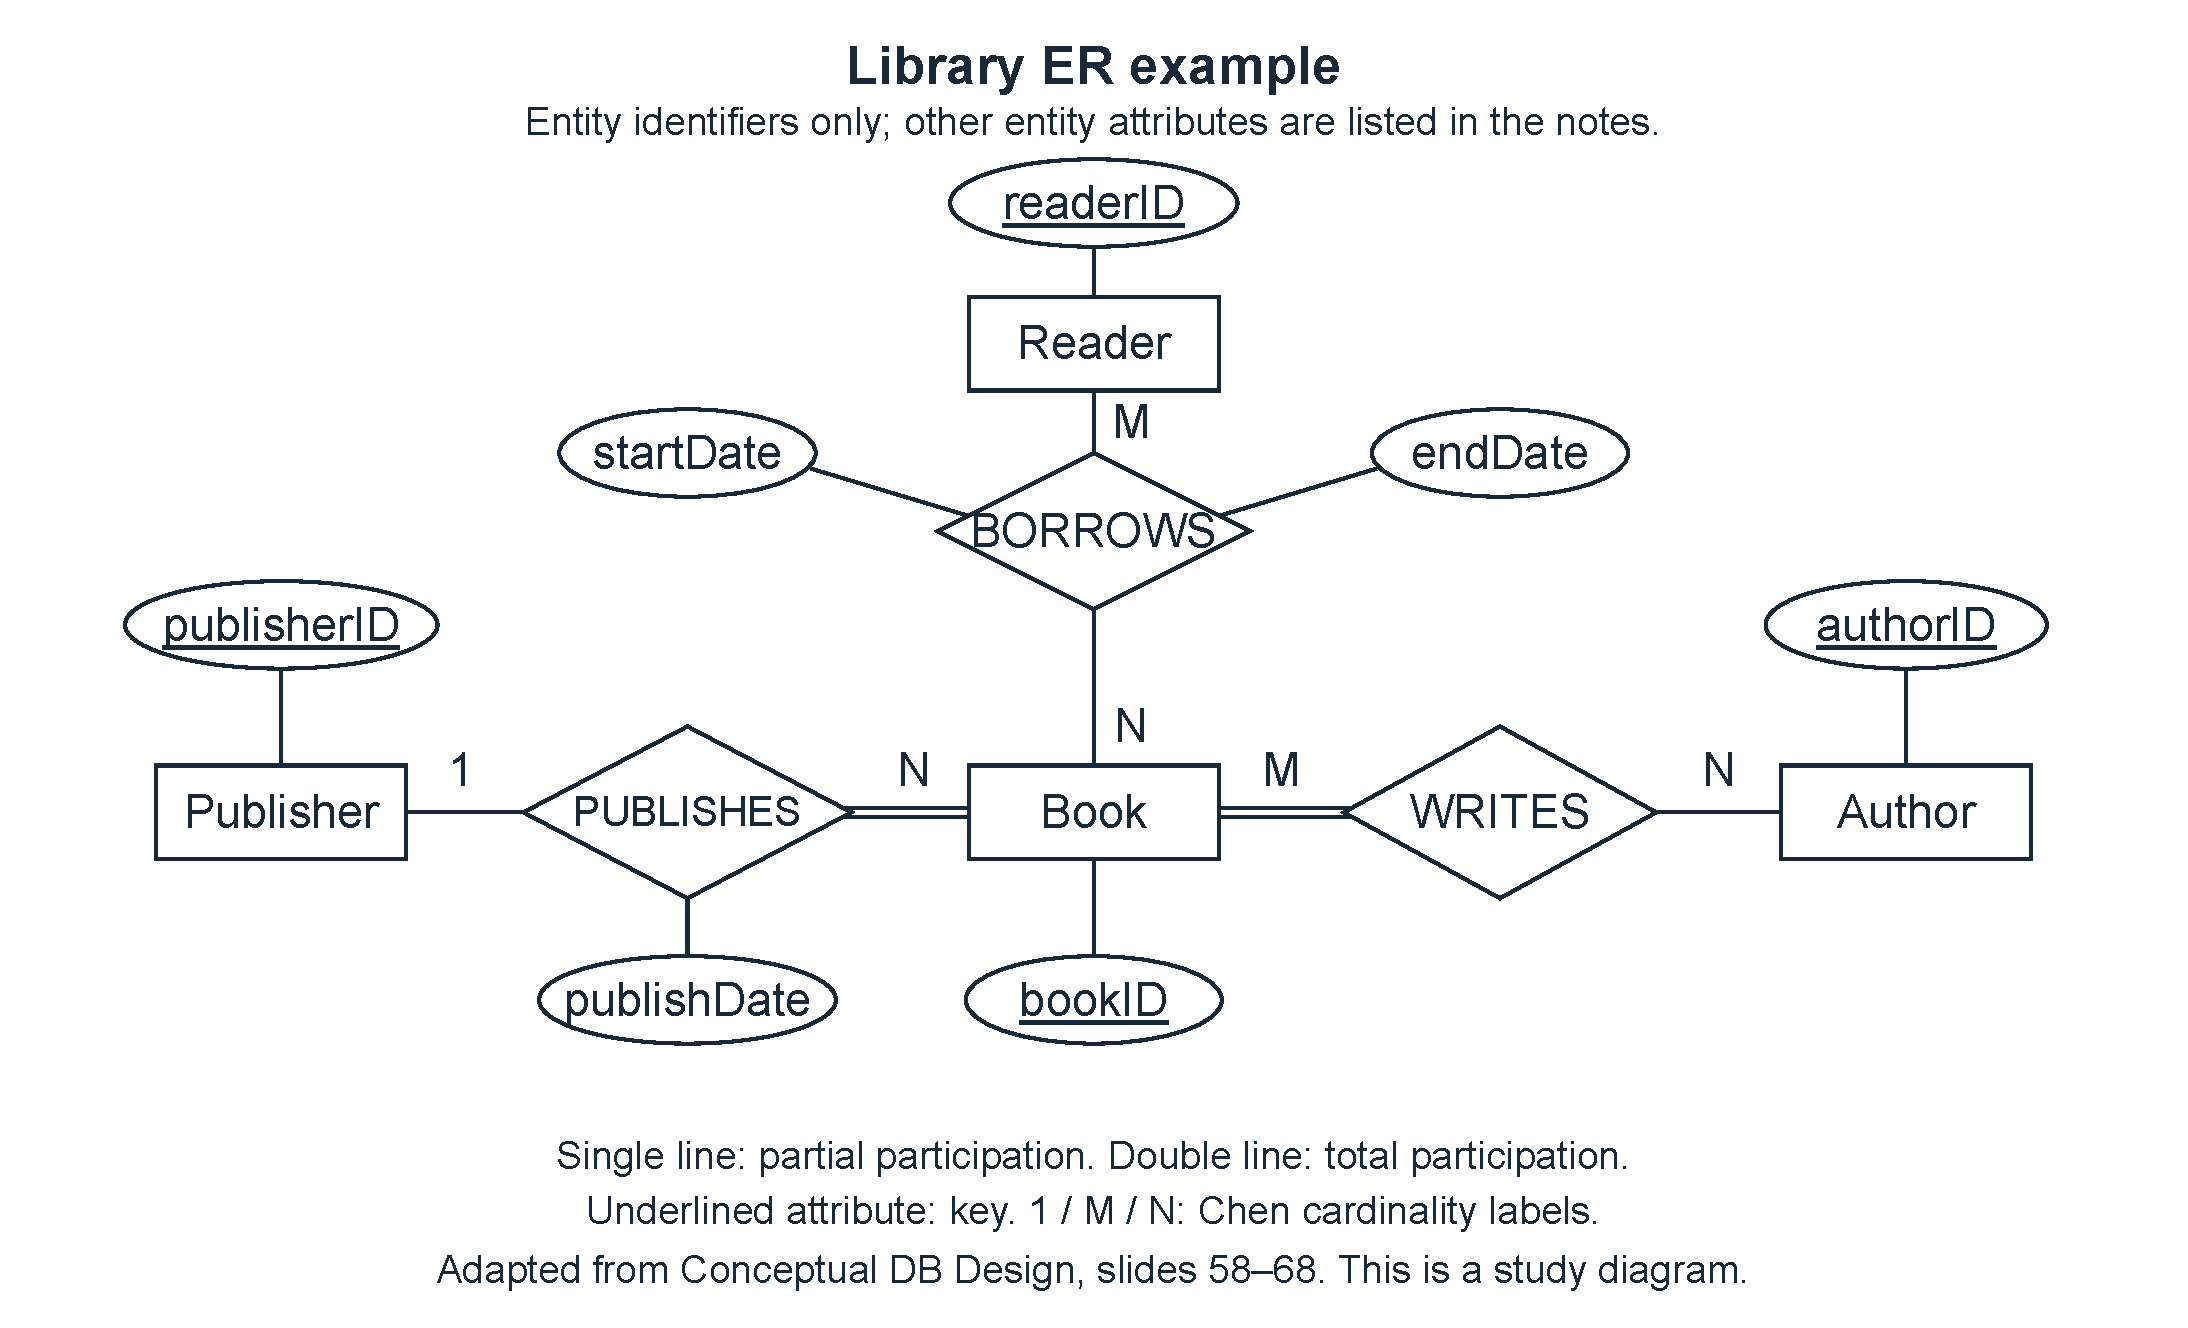
\includegraphics[keepaspectratio,alt={Library ER study diagram: identifiers, relationship attributes, cardinalities, and participation}]{figures/02_er_modelling_example.pdf}}
\caption{Library ER study diagram: identifiers, relationship attributes, cardinalities, and participation}
\end{figure}

This redraw shows \textbf{only key attributes of entities}. Other entity attributes appear in the table above. The date attributes belong to relationship diamonds. Check the double lines from Book to PUBLISHES and WRITES, then the single lines at both ends of BORROWS, to distinguish the three participation rules.

\textbf{Model boundary (explanatory supplement):} a regular binary relationship instance is determined by its participating entity pair. If the application must preserve separate records of the same Reader repeatedly borrowing the same Book, dates attached to a Reader--Book relationship alone do not distinguish those repeated events. Introduce a Loan entity and specify how it is identified. The lecture example does not fully develop this history requirement; this supplement is not an additional compulsory answer imposed on the original exercise.

\subsection{11. A procedure for modelling written requirements}\label{02_er_modelling_en-a-procedure-for-modelling-written-requirements}

Source: slides 54--55 and 58--70; the steps below organize the lecture material into a working procedure.

\begin{enumerate}
\def\labelenumi{\arabic{enumi}.}
\tightlist
\item
  \textbf{Read all requirements, then identify entities.} Define each candidate type and decide which objects require independent identification.
\item
  \textbf{List and classify attributes.} Identify composite, multivalued, derived, and potentially missing information; find the entity keys.
\item
  \textbf{Check weak entities.} Is a number unique only within an owner? Record the owner, partial key, and full identification chain.
\item
  \textbf{Name each relationship.} Several relationships may connect the same types; label roles when a type participates more than once.
\item
  \textbf{Write minima and maxima in both directions.} Derive cardinality and participation from them; a bare ``1:N'' is insufficient.
\item
  \textbf{Place relationship attributes.} Decide whether each property describes one object or an association among participants.
\item
  \textbf{State rules the diagram cannot fully express.} Examples include MANAGES pairs being WORKS\_AT pairs, time ordering, and numbering sequences. Label assumptions where requirements are silent.
\item
  \textbf{Read the whole diagram back into sentences.} Check every box, connection, and label against the requirements for both missing and unjustified constraints.
\end{enumerate}

Slide 55 gives four design criteria: correctness, completeness, consistency, and readability. Several designs may be reasonable, but ``no single best design'' does not excuse missing constraints.

\subsection{12. Common distinctions}\label{02_er_modelling_en-common-distinctions}

\begin{longtable}[]{@{}
  >{\raggedright\arraybackslash}p{(\linewidth - 2\tabcolsep) * \real{0.5000}}
  >{\raggedright\arraybackslash}p{(\linewidth - 2\tabcolsep) * \real{0.5000}}@{}}
\toprule\noalign{}
\begin{minipage}[b]{\linewidth}\raggedright
Pair
\end{minipage} & \begin{minipage}[b]{\linewidth}\raggedright
Distinction
\end{minipage} \\
\midrule\noalign{}
\endhead
\bottomrule\noalign{}
\endlastfoot
Entity / entity type / entity set & One object / common structural definition / current collection \\
Simple / single-valued & Whether meaningful subdivision is needed / whether one value is allowed at a time \\
Composite attribute / composite key & An attribute with components / several attributes jointly identifying an entity \\
Composite / multivalued & Components of one value / several values for one entity \\
Superkey / candidate key & Unique / unique with no redundant attribute \\
Partial key / full identifier & Unique within one owner / complete identification with owner context \\
Weak entity / existence dependency & Weakness requires identification through an owner; existence dependency alone is insufficient \\
Cardinality / participation & Maximum related entities / whether every entity must participate \\
Double line / double oval & Total participation / multivalued attribute \\
Entity attribute / relationship attribute & Property of an object / property of an association \\
ER relationship / relational relation & Association in a conceptual model / a relation (table) in the relational model \\
\end{longtable}

\subsection{13. Revision checklist and short-answer language}\label{02_er_modelling_en-revision-checklist-and-short-answer-language}

These are learning goals, not a formal practice test or an official mark allocation.

\begin{itemize}
\tightlist
\item[$\square$]
  Distinguish an entity, entity type, and entity set using examples.
\item[$\square$]
  Classify attributes separately by decomposition, number of values, and derivation.
\item[$\square$]
  Explain why a minimal candidate key need not have the smallest number of attributes.
\item[$\square$]
  Give a weak entity's owner, partial key, identifying relationship, and full identifier.
\item[$\square$]
  State minimum and maximum participation counts in both directions for every relationship.
\item[$\square$]
  Use key underlines, double rectangles, double diamonds, double ovals, and single/double lines correctly.
\item[$\square$]
  Explain why time fractions and borrowing dates can be relationship attributes.
\item[$\square$]
  Translate the library diagram back into requirements and identify its boundary for repeated borrowing history.
\item[$\square$]
  State assumptions explicitly when a constraint cannot be determined from the requirements.
\end{itemize}

Useful short-answer formulations:

\begin{quote}
An entity type describes a collection of entities that share the same attributes.
\end{quote}

\begin{quote}
A candidate key is a minimal superkey: no proper subset is still a superkey.
\end{quote}

\begin{quote}
A weak entity is identified by its owner's identifier together with its partial key.
\end{quote}

\begin{quote}
Cardinality constrains the maximum number of related entities; participation specifies whether every entity must participate.
\end{quote}

\begin{quote}
Total participation requires every entity of that type to participate in at least one instance of the relationship.
\end{quote}

\begin{quote}
The attribute belongs to the relationship because its value describes a particular combination of participating entities.
\end{quote}

\subsection{Sources and preparation record}\label{02_er_modelling_en-sources-and-preparation-record}

\begin{itemize}
\tightlist
\item
  Lecturer's deck: \href{../../../slides/Week\%201B\%20-\%20Conceptual\%20DB\%20Design.pptx}{Week 1B - Conceptual DB Design.pptx}, 70 slides. Text was read; diagrams on slides 35--36, 45, 47, 51, 53, 57, and 68 were visually inspected. The library example follows slides 58--68; the SVG is a study redraw omitting non-key entity attributes.
\item
  Scope: \href{../../../syllabus/CSC5041_Teaching_Plan.pdf}{CSC5041\_Teaching\_Plan.pdf}, page 1, Week 2, and page 2, Tutorial 1. Supporting exercise: \href{../../../slides/Tutorial1.pdf}{Tutorial1.pdf}, page 1, Question 1(a)--(b). This chapter supplies neither a complete tutorial solution nor a practice paper.
\item
  Clarifications concerning attribute classification, partial keys, roles, ternary decomposition, and repeated borrowing are identified in the relevant sections. They are not presented as verbatim lecture statements.
\item
  LaTeX edition prepared on 20 October 2026; original evidence status is retained. No new database execution is claimed.
\item
  Input SHA-256: ER deck \texttt{\seqsplit{1f2bc2b2242208b0d3f0c650341521c65cba833cffe5da82fc27d0ddef7fc734}}; Tutorial 1 \texttt{\seqsplit{316e8b6bb9581a5ecae3fb2f449e395a4ea8a19b4ee16c4191fc20a6079d2c44}}; syllabus teaching plan \texttt{\seqsplit{31380a7fe6504e46541b6db0bb2f24859c69188bfeb9681dca73354ebeb68295}}. These are the versions read this turn, rather than hashes copied from Chapter 01.
\end{itemize}
